% Intro chapter
\pagenumbering{arabic}
\chapter{Introduction}

% abstract
\begin{tcolorbox}[title=Abstract,colbacktitle=white!80!black,coltitle=black,arc=0mm,boxrule=0.1mm]
Shape memory alloys (SMAs) have been adapted as sensors or actuators in a number of aerospace technologies. SMAs can exhibit unique hysteretic behaviours due to the non-convex nature of their free energy functions. We begin with a discussion of SMAs and their properties, followed by a decription of variational approaches to modeling SMAs in Chapter \ref{ch:2}. Next, we offer some examples of the numerous applications of SMAs as sensors and actuators in the aerospace industry, including present and future uses. Finally, we briefly outline the formalism behind a continuous time model relevant to numerical simulation and discuss a computational model of Nitinol.\\

{\footnotesize\hspace{5mm}\textbf{Key Words:} Shape-Memory Alloys, Smart Materials, memory property, strain, stress, polycristalline, hysteresis.} %\todo{what else? bring it on}
\end{tcolorbox}

% beginning of text body
\begin{multicols}{2}
\section{Historical Background}
In their article \underline{Memory Metal} \cite{kauffman1993memory},  George B. Kauffman and Issac Mayo tell about how scientist and engineer William J. Buehler discovered the peculiar ``memory" property exhibited by a nickel-titanium alloy, under conditions which likely describe a large portion of scientific discoveries: ``A lot of work and a little luck". After returning from World War II, Buehler started experimenting in his lab with different compounds chosen from the book \underline{\textit{The Constitution of Binary Alloys}} to find a fatigue-, impact-, and heat-resistant alloy to be used in the cone of a missile.\cite{kauffman1993memory} After working a considerable amount of time in his laboratory (according to the article \underline{Metal with Memory} \cite{mayometalwithmemory}, he worked from 4:00AM to 11:00PM in an effort to seek solace in his lab during his separation from his wife), Buehler realized that one of the alloys (nickel-titanium, now commonly known as Nitinol) seemed to be considerably more durable than the rest that he tested. Later on, in a demonstration of durability shown on strips of metal alloys, he folded the strips into an accordion shape and passed it around among the attendees for them to observe this durability themselves. After one attendee, Dr. David S. Muzzey tried heating the strip with his pipe lighter, to everyone's surprise, the strip stretched out back to its original shape \cite{kauffman1993memory}. This curious discovery of the so-called ``memory property" (observed in other materials as well) was then studied by many scientists and engineers. Today, shape-memory alloys, which fall under the class of smart materials, are used in numerous areas such as aerospace, robotics and (quite ironically, given Buehler's initial goal) medicine. 

\section{Properties of Shape Memory Alloys}\label{sec:properties}
The unique nature of SMAs arises from their ability to recover from up to 10\% strains due to temperature or stress-induced deformations. This is because SMAs can exist in two distinct, thermodynamically stable phases: austenite and martensite \cite{smith2005smart}. Transitions between these two phases account for two key properties of SMAs, namely the \textit{shape memory} and \textit{pseudo-elastic} effects.

Firstly, consider the cooling and reheating of a SMA sample in the absence of any applied load. At a high temperature, the sample is in the cubic austenite phase. Upon cooling, the lattice reconfigures to the twinned martensite phase, as depicted in figure \ref{fig:phases} below. When reheated, the sample returns to the austenite phase. Hence, the SMA is able to ``remember" its original configuration in the austenite phase. We denote the temperatures at which the phase transitions begin and end as $M_s$, $M_f$, $A_s$, and $A_f$ for the martensite (M) and austenite (A) phases, respectively \cite{smith2005smart}. The subscripts $s$ and $f$ are used to distinguish between the temperatures at which the phase transformations ``start" and ``finish".  It should be noted here that depending on the alloy used, these temperatures can be tuned to values suited to a particular application.

\begin{figure}[H]
    \centering
    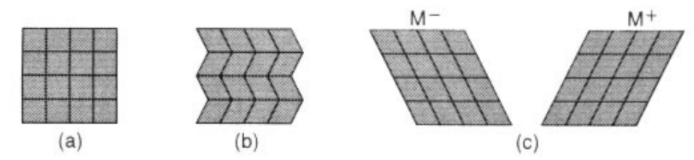
\includegraphics[scale=0.39]{._figures/SMA phases.png}
    \caption[Schematic representation of the solid SMA phases]{Schematic representation of the three phases of a shape memory alloy: (a) austenite, (b) twinned martensite, and (c) detwinned martensite variants.}
    \label{fig:phases}
\end{figure}

If an external stress is applied to the sample, the resulting phase transformation is dependent upon the temperature of the environment. If the temperature is greater than $A_f$, then the sample is initially in the austenite phase and exhibits an approximately linear (elastic) stress-strain relationship. Once the stress attains a critical value $\sigma_M$, it becomes energetically favourable for the sample to transition to the detwinned martensite phase \cite{smith2005smart}. When the stress is decreased, the stress-strain curve again becomes approximately linear until the lower critical value of $\sigma_A$ is reached. At this point, the material begins to revert to the austenite configuration and the sample fully recovers its initial shape. Conversely if the temperature is below $M_f$, the material begins in the twinned martensite state and will not return to its austenite form. Instead, it retains some `plastic' or residual strain upon unloading. The sample must be heated above $A_f$ to undergo complete shape recovery. A graphical representation of these two cases is shown in figure \ref{fig:stress_strain} below.

\begin{figure}[H]
    \centering
    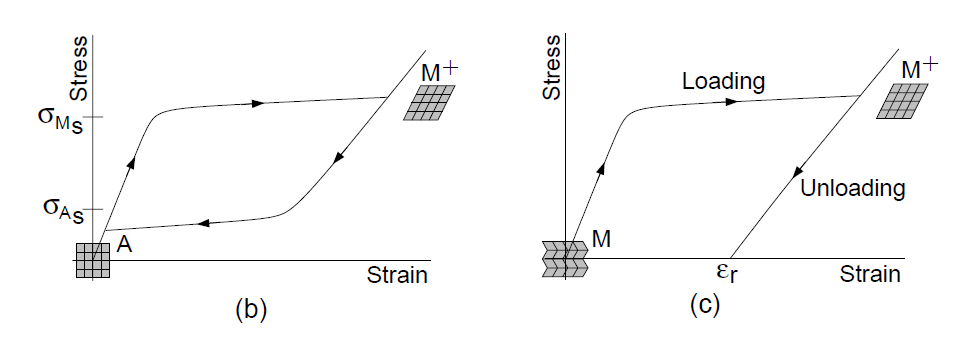
\includegraphics[scale=0.33]{._figures/Smith Fig1-18.png}
    \caption[Stress-strain curves subject to external loading for $T>A_f$]{Adapted from figure 1.18 in \cite{smith2005smart}. In (b) we see the stress-strain curve subject to external loading/unloading when $T > A_f$. (c) depicts the curve when $T < M_f$. Notice that in (c), the sample begins in the twinned martensite ($M$) state and retains some residual strain $\varepsilon_r$ upon unloading.}
    \label{fig:stress_strain}
\end{figure}

The ability of an SMA to return to its original shape upon removal of external stress in the high-temperature regime (Figure \ref{fig:stress_strain} (b)), is known as the \textit{pseudoelastic} or \textit{superelastic} effect.

Materials that have been classified as SMAs (in addition to NiTi) include alloys of: Copper-aluminium- nickel (CuAlNi), copper-zinc-aluminium (CuZnAl), and iron- manganese-silicon (FeMnSi) \cite{smith2005smart}. Nitinol is perhaps the most well-known and widely used of these.

\section{Exhibition of Hysteretic Behavior in Shape Memory Alloys}
Many of the properties that make shape memory alloys (SMAs) a topic of interest are classified under the phenomenon called hysteresis. Along with SMAs, some of the various systems that exhibit hysteretic behavior are cell signaling, an electronic comparator or a beam in a magnetic field \cite{morris2011hysteresis}. In the article named \underline{What is Hysteresis?}, Morris points out the lack of a general definition for this phenomenon and suggests a definition based on the system dynamics and operation in contrast to the existing definitions that are specific to different classes of systems \cite{morris2011hysteresis}. 

The term \emph{hysteresis} (which roughly translates from Greek as ``to lag behind") was first used in the paper \underline{Experimental Researches in Magnetism} \cite{morris2011hysteresis}. The core properties of SMAs (and other smart materials) are results of hysteretic behaviors, namely its memory property and the \emph{rate independence} of operation. These materials transform one form of energy into another. Temperature driven SMAs turn thermal energy into mechanical energy while magnetostrictives (including magnetic SMAs) transform magnetic work into mechanical energy, yet the two systems have the same inherent memory and rate independence properties. Qualitatively, rate independence means that the output of the system is only dependent on the system input and not on how quickly the input is being varied \cite{morris2011hysteresis}. The complete dependence of the input-output graph on the input makes it appear as if the system ``remembers" its initial state, giving rise to the \emph{memory property}. 


\subsection{Analyzing the Hysteretic Behavior of a Magnetostrictive Material}
In an effort to construct a more abstract definition of hysteresis, Morris examines various systems that are said to exhibit hysteresis; one of them being the response of a magnetostrictive material to an external magnetic field \cite{morris2011hysteresis}. In the model, the magnetostrictive material (some examples of which include the alloys Terfenol-D and Galfenol) is thought to be composed of magnetic dipoles. Qualitatively, the Gibbs energy function for dipoles of different values of external magnetic fields are given. When there is no field applied, the system has a symmetric energy function. As the strength of the external magnetic field is increased, the energy function tends towards a polarized, asymmetric configuration favoring one stable point over the other until only one equilibrium point remains (see Figure \ref{fig:austenitemartensite}). Following Hamilton's principle, ``Between fixed times $a$ and $b$, a system moves along the trajectory that makes stationary the action integral over all admissible trajectories"\cite{coursenotes}. The symmetry of the system is tunable and the system is naturally driven to the equilibrium points, making it possible (in a sense) to ``initialize" the material with each dipole setting being one of the two equilibrium points. This uniqueness that gives rise to the memory property of magnetostrictive materials is ultimately a result of the energy function of the dipoles being non-convex. By Proposition 2.15 of the course notes, if $J$ is convex, then any stationary point of $J$ in $D$ minimizes $J$ on $D$.\cite{coursenotes} Hence, if $J$ were convex everywhere, there could not be a local maximum in between the two stable equilibria (or in fact, anywhere) to give rise to an adjustable binary system. The state possessing high symmetry corresponds to austenite and the state with lower symmetry corresponds to martensite \cite{smith2005smart}.

\begin{figure}[H]
    \centering
    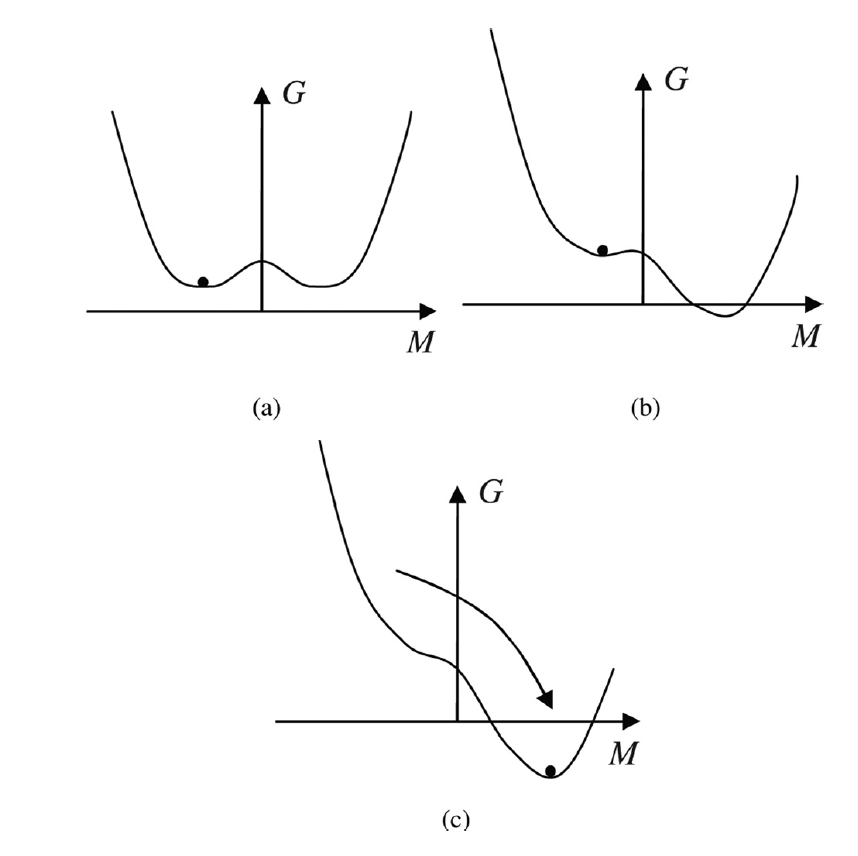
\includegraphics[scale=0.33]{._figures/austenitemartensite.png}
    \caption[Equilibria of the SMA energy function in a magnetic field]{The value of $H_0$ is 0 in (a) and is gradually increased. The system starts favoring one equilibrium point over the other in (b), until there is only one equilibrium left in (c). \cite{morris2011hysteresis}}
    \label{fig:austenitemartensite}
\end{figure}

Before building a macro model, it is insightful to first describe the mathematics on the micro scale as in the Homogenized Energy approach (see Chapter \ref{ch:2} for more detail). A dipole in a magnetostrictive material is governed by the minimization of the Gibbs free energy, which is defined through the function $f(M)$ and ultimately through the Helmholtz energy, defined in \cite{morris2011hysteresis} as:

\begin{equation}\label{111}
    \Psi(m,\varepsilon)=\frac{1}{2}y\varepsilon^2-Y\gamma_1\varepsilon M^2+f(M),
\end{equation}
where 

\begin{equation}\label{112}
f(M)=\begin{cases} 
      \frac{\mu_0\eta}{2}(M+M_R)^2, & M\leq -M_I, \\
      \frac{\mu_0\eta}{2}(M_R-M_I)(M_R-\frac{M^2}{M_I}) & \abs{M}< M_I, \\
      \frac{\mu_0\eta}{2}(M-M_R)^2, & M\geq M_I.
   \end{cases}
\end{equation}
In equations (\ref{111}) and (\ref{112}) , M is the magnetization of the dipole, $\varepsilon$ is the total strain, and $M_R$ $\eta $, $\gamma_1$ and Y are physical constants. $M_R$ is determined experimentally and plays a crucial mathematical role, as $\pm M_R$ give the deviation of the equilibrium points from $\frac{H_0}{\eta}$, which create the two ``states" for the case with no applied magnetization. The presence of this physical constant is a key property that makes smart materials fine tunable.
\begin{equation}\label{113}
    G(H_0,M,\sigma,\varepsilon)=\Psi(m,\varepsilon)-\mu_0 H_0 M
\end{equation}
 To find the equilibrium points, the Gibbs free energy given in (\ref{113}) is partially differentiated with respect to the magnetization M (for the case where $\abs{M}<M_I $) to yield the locations of equilibria and the critical value $H_c$ after which the system posseses only one equilibrium. This calculation gives:
 \begin{align}
M^*_+=\frac{H_0}{\eta}+M_R, \label{114}\\
M^*_-=\frac{H_0}{\eta}-M_R,\\
H_c=\eta(M_R-M_I),\label{115}
\end{align}
according to \cite{morris2011hysteresis}.
With these expressions, it is now clear how to shift the system from two equally favored equilibria to only one on the micro scale by vayring the external field. If the system can respond to changes in the field fast enough (the idealization of which is called rate-independence), it has the potential to exhibit the exotic hysteretical behaviors. Having set up an abstract mathematical background, following the analysis of this example and various others, the paper suggests a general definition as follows:
``A hysteretic system is one which has (1) multiple stable equilibrium points and (2) dynamics that are considerably faster than the time scale at which inputs are varied." \cite{morris2011hysteresis} After establishing the model on the micro scale, material behaviour on the macro scale can be investigated by way of homogenization techniques or by other means.

\end{multicols}